\documentclass{ugmskripsi}

\usepackage{amsmath}
\usepackage{booktabs}
\usepackage[justification=centering, font=bf]{caption}
\usepackage{array}
\newcolumntype{L}[1]{>{\raggedright\let\newline\\\arraybackslash\hspace{0pt}}p{#1}}
\renewcommand{\arraystretch}{1.2}

\usepackage{courier}
\usepackage{color}
\usepackage{listings}
\lstset{
	basicstyle=\footnotesize\ttfamily,
	numbers=left,
 	numberstyle=\scriptsize,
	frame=tb,
    aboveskip=10pt,
	tabsize=4,
	columns=fixed,
	showstringspaces=false,
	showtabs=false,
	keepspaces,
	commentstyle=\color{red},
	keywordstyle=\color{blue}
}

%------------------------------------------------------------------------------
% Title
%------------------------------------------------------------------------------
\titleind{PENGENALAN AKTIVITAS MANUSIA MENGGUNAKAN SENSOR PADA SMARTPHONE DENGAN CONVOLUTIONAL NEURAL NETWORK DAN LONG SHORT-TERM MEMORY}

\titleeng{HUMAN ACTIVITY RECOGNITION USING SMARTPHONE SENSORS WITH CONVOLUTIONAL NEURAL NETWORK AND LONG SHORT-TERM MEMORY}

%------------------------------------------------------------------------------
% Author Details
%
% FIXME:
% - Exam date
% - Supervisor
% - Examiner
%------------------------------------------------------------------------------
\fullname{ILHAM IMADUDDIN}
\idnum{13/352625/PA/15682}
\examdate{... 2017}
\degree{Sarjana Sains}
\yearsubmit{2017}
\program{Elektronika dan Instrumentasi}
\headprogram{Drs. Agus Harjoko M.Sc., Ph.D}
\dept{Ilmu Komputer dan Elektronika}
\firstsupervisor{Raden Sumiharto S.Si., M.Kom}

%------------------------------------------------------------------------------
% Content
% TODO:
% - Acknowledment
% - Prakata
%
%------------------------------------------------------------------------------
\begin{document}

\cover{}
\titlepageind{}
% \approvalpage{}
\declarepage{}

% \acknowledment{}
% \begin{flushright}
%     Untuk Ibu dan Apa.
% \end{flushright}

\preface
Prakata

\tableofcontents
\listoftables
\listoffigures

\begin{abstractind}
    Pengenalan aktivitas manusia adalah salah satu masalah yang berusaha diselesaikan dalam pengembangan lingkungan cerdas. Agar dapat digunakan secara praktis, berbagai percobaan dilakukan untuk mengenali aktivitas manusia menggunakan sensor yang tertanam pada ponsel cerdas. Beberapa metode pembelajaran mesin telah digunakan untuk mengklasifikasikan aktivitas dengan cukup baik, namun terhambat oleh kesulitan pemilihan representasi data yang terbaik. Pada penelitian ini dilakukan penyusunan sistem pengenalan aktivitas manusia berdasarkan data sensor akselerometer dan giroskop dari ponsel cerdas dengan \textit{deep learning} untuk pencarian representasi data secara otomatis.

    Model klasifikasi dibuat dengan menyusun lapisan-lapisan \textit{convolutional neural network} dan \textit{long short-term memory} untuk mengekstrak fitur dari data sensor. Fitur-fitur tersebut kemudian diklasifikasi dengan lapisan \textit{softmax} untuk menghasilkan enam aktivitas yang berbeda, yaitu duduk, berdiri, berjalan, berlari, menaiki tangga dan menuruni tangga. Jaringan tersebut diregulasi dengan \textit{dropout} untuk mencegah \textit{overfitting}.

    Pengujian sistem dilakukan untuk mengoptimasi \textit{hyperparameter} model, mengukur akurasi klasifikasi \textit{online} dan mengukur kecepatan klasifikasi pada ponsel cerdas. Hasil pengujian dengan \textit{hyperparameter} optimal menunjukkan tingkat akurasi klasifikasi \textit{offline} sebesar 93,15\% dan klasifikasi \textit{online} sebesar 90,92\%. Pengujian pada tiga ponsel cerdas yang berbeda juga menunjukkan waktu komputasi yang cukup cepat untuk klasifikasi secara \textit{realtime}.

    \bigskip
    Kata-kata kunci: \textit{deep learning}, optimasi \textit{hyperparameter}, ekstraksi fitur
\end{abstractind}

\begin{abstracteng}
    \itshape
    Human activity recognition is an unsolved problem in the development of smart environment. Researchers have been using embedded sensor on smartphone to practically recognize human activity. Several machine learning method have been used with good result, but it requires the researcher to hand-design the best data representation. This research is an attempt to create a human activity recognition system based on accelerometer and gyroscope data from smartphone with deep learning to find an optimal data representation.

    A classification model is created by stacking layers of convolutional neural networks and long short-term memory to extract abstract features from sensor data. Those features are classified with a softmax layer to predict six different activities: sit, stand, walk, jog, walking upstairs and walking downstairs. The network is regulated with dropout to prevent overfitting.

    The system are tested to optimize the model's hyperparameter, to measure accuracy of online classification and to measure computation time on smartphones. A test with optimized hyperparameter resulted in 93.15\% accuracy on offline classification and 90,92\% accuracy on online classification. Computation time are tested on three different smartphone, the result shows that the computation time is fast enough to do classification in realtime.

    \bigskip
    Keywords: deep learning, hyperparameter optimization, feature extraction
\end{abstracteng}

\chapter{PENDAHULUAN}

\section{Latar Belakang Masalah}
Pengenalan aktivitas manusia adalah salah satu bidang yang penting dalam pengembangan lingkungan cerdas. Manfaatnya berpotensi untuk meningkatkan kemampuan lingkungan cerdas dalam membantu aktivitas manusia. Salah satu metode untuk mengenali aktivitas adalah menggunakan sensor pada tubuh manusia untuk membaca gerakan tubuh.

Berbagai penelitian dilakukan untuk mengenali aktivitas dari gerakan tubuh. Pada awalnya pengambilan data dilakukan dengan sensor yang digunakan pada beberapa bagian tubuh yang berbeda, seperti pergelangan tangan, lengan, dada, paha, dan pergelangan kaki. Proses pembelajaran mesin dilakukan pada komputer yang terpisah untuk mengklasifikasikan data sensor menjadi aktivitas. Namun pendekatan tersebut memiliki kesulitan untuk diimplementasikan pada masyarakat luas karena pengguna perlu menggunakan beberapa perangkat eksternal.

Seiring dengan berkembangnya teknologi, berbagai penelitian pun dilakukan dengan memanfaatkan sensor-sensor yang tertanam pada ponsel cerdas. Ponsel cerdas dilengkapi dengan beberapa sensor seperti akselerometer, giroskop, GPS dan kamera yang dapat dimanfaatkan untuk mengumpulkan informasi mengenai perangkat dan konteksnya. Selain itu ponsel cerdas juga memiliki kemampan komputasi yang tinggi yang memungkinkan kita untuk memproses tugas komputasi secara lokal.

Beberapa metode pembelajaran mesin telah digunakan dan menghasilkan klasifikasi aktivitas yang cukup baik. Penelitian yang dilakukan oleh \Textcite{Chiang-201413} menghasilkan tingkat akurasi terbaik ketika menggunakan metode \textit{Support Vector Machine (SVM)}, sedangkan penelitian yang dilakukan oleh \Textcite{shoaib-2013} menunjukkan bahwa metode terbaik berbeda-beda untuk setiap aktivitas. Perbedaan ini terjadi karena masing-masing peneliti memilih representasi data yang berbeda, sedangkan performa suatu algoritma sangat bergantung pada representasi dari data yang digunakan \Parencite{Goodfellow-2016}. Selain itu salah satu kesulitan dalam klasifikasi aktivitas adalah setiap orang melakukan aktivitas dengan cara yang beragam. Penelitain yang dilakukan oleh \Textcite{tapia-2007} menghasilkan tingkat akurasi 94,6\% pada pelatihan yang bergantung pada subjek, namun menurun drastis menjadi 56,3\% pada pelatihan yang independen terhadap subjek.

\textit{Deep learning} adalah salah satu bidang pembelajaran mesin yang populer dalam beberapa tahun terakhir. Berbagai masalah yang semula sulit bagi metode pembelajaran mesin tradisional kini dapat diselesaikan dengan baik menggunakan \textit{deep learning}. Berbeda dengan metode pembelajaran mesin tradisional yang memerlukan pemilihan representasi data secara manual, \textit{deep learning} mampu mencari representasi data secara otomatis. \textit{Deep learning} merepresentasikan suatu konsep yang kompleks sebagai rangkaian konsep-konsep yang lebih sederhana. Kemampuan ini menjadi salah satu alasan \textit{deep learning} memiliki performa yang lebih baik dari metode pembelajaran mesin lainnya.

Dalam penelitian ini dirancang sebuah sistem pengenalan aktivitas manusia yang melengkapi kekurangan penelitian-penelitian sebelumnya. Pengenalan aktivitas dilakukan berdasarkan sensor akselerometer dan giroskop yang tertanam pada ponsel cerdas. Data sensor tersebut diklasifikasi dengan \textit{Convolutional Neural Network (CNN)} dan \textit{Long Short Term Memory (LSTM)} untuk mengenali enam aktivitas sederhana, yaitu duduk, berdiri, berjalan, berlari, menaiki tangga dan menuruni tangga.

\section{Rumusan Masalah}
Berdasarkan latar belakang di atas, dirumuskan bagaimana cara melakukan pengenalan aktivitas manusia berdasarkan data sensor dari ponsel cerdas.

\section{Batasan Masalah}
Penelitian ini memiliki batasan masalah sebagai berikut:

\begin{enumerate}
    \item Ponsel cerdas yang digunakan bersistem operasi Android, memiliki sensor akselerometer dan giroskop.
    \item Pengenalan aktivitas dibatas menjadi enam aktivitas sederhana, yaitu duduk, berdiri, berjalan, berlari, menaiki tangga dan menuruni tangga.
    \item Pada saat proses pengenalan, ponsel cerdas ditempatkan pada saku celana dengan posisi acak.
\end{enumerate}

\section{Tujuan Penelitian}
Penelitian ini bertujuan untuk membuat purwarupa sistem yang dapat melakukan pembelajaran dengan CNN dan LSTM untuk mengenali aktivitas manusia berdasarkan sensor akselerometer dan giroskop yang tertanam pada ponsel cerdas.

\section{Manfaat Penelitian}
Manfaat penelitian ini adalah menghasilkan sebuah model klasifikasi aktivitas manusia yang dapat digunakan untuk mengingkatkan kemampuan lingkungan cerdas dalam memantau dan membantu aktivitas manusia.

\section{Metodologi Penelitian}
Penelitian ini dilakukan dalam beberapa tahap yang meliputi studi pustaka dan literatur, diskusi dan konsultasi, perancangan sistem, implementasi serta pengujian. Berikut metodologi yang dilakukan dalam penelitian ini:

\begin{enumerate}
    \item Studi pustaka dan literatur dilakukan untuk mengkaji penelitian, buku, karya tulis ilmiah dan jurnal yang berkaitan dengan penelitian ini.
    \item Diskusi dan konsultasi dilakukan bersama dosen pembimbing untuk mempelajari lebih lanjut topik yang dibahas. Pada tahap ini dicari metode-metode yang sebaiknya digunakan untuk menyelesaikan masalah dalam penelitian ini.
    \item Perancangan sistem dibuat sesuai dengan analisis kebutuhan. Rancangan yang dibuat terdiri dari model klasifikasi, proses pelatihan model, proses klasifikasi pada ponsel cerdas, dan rencana pengujian.
    \item Implementasi dibuat untuk rancangan sistem yang telah disusun. Pembuatan dan pelatihan model diimplementasikan dengan bahasa Python pada sistem operasi Ubuntu 16.04, sedangkan sistem klasifikasi \textit{online} diimplementasikan pada ponsel cerdas dengan sistem operasi Android menggunakan bahasa Java. Keduanya memanfaatkan TensorFlow sebagai pustaka komputasi numerik.
    \item Pengujian dilakukan untuk mengetahui kemampuan klasifikasi dari model yang telah dibuat. Parameter yang diuji adalah akurasi klasifikasi \textit{offline}, akurasi klasifikasi \textit{online} dan kecepatan klasifikasi pada ponsel cerdas.
\end{enumerate}

\section{Sistematika Penulisan}
Sistematika penulisan yang digunakan dalam laporan penelitian ini adalah sebagai berikut:

\subsubsection{BAB I PENDAHULUAN}
Bab ini berisi latar belakang penelitian, rumusan masalah, batasan masalah, tujuan penelitian, manfaat penelitian, metodologi penelitan dan sistematika penulisan.

\subsubsection{BAB II TINJAUAN PUSTAKA}
Bab ini memuat uraian penelitian-penelitian terkait yang sudah pernah dilakukan dalam penelitian lain dan hubungannya dengan masalah penelitian yang sedang dilakukan.

\subsubsection{BAB III DASAR TEORI}
Bab ini berisi teori-teori dasar yang mendukung penelitan yang akan dilakukan.

\subsubsection{BAB IV ANALISIS DAN PERANCANGAN SISTEM}
Bab ini menjelaskan analisis kebutuhan dan perancangan sistem yang akan digunakan. Pada bab ini dibahas pembuatan model klasifikasi, proses pelatihan model dari data latih, pengaplikasiannya pada ponsel cerdas serta rencana pengujian sistem.

\subsubsection{BAB V IMPLEMENTASI}
Bab ini membahas implementasi dari rancangan sistem yang telah dibuat, meliputi implementasi model klasifikasi, implementasi pengambilan dan pengondisian data, implementasi klasifikasi pada ponsel cerdas dan implementasi pengujian.

\subsubsection{BAB VI HASIL DAN PEMBAHASAN}
Bab ini menjelaskan hasil dari pengujian akurasi klasifikasi \textit{offline}, akurasi klasifikasi \textit{offline} dan kecepatan klasifikasi pada ponsel cerdas.

\subsubsection{BAB VII PENUTUP}
Bab ini berisi kesimpulan dari penelitian yang telah dilakukan serta saran untuk pengembangan sistem selanjutnya.

\chapter{TINJAUAN PUSTAKA}

Dalam pengenalan aktivitas, berbagai jenis teknologi pengindraan telah dieksplorasi untuk meningkatkan pengenalan dan adaptasi ke berbagai skenario aplikasi. Pada umumnya, pengenalan aktivitas dapat dikelompokkan menjadi tiga kategori: pendekatan berbasis \textit{vision}, pendekatan berbasis sensor interaksi lingkungan, dan pendekatan berbasis \textit{wearable sensor} \citep{wang-2016}. Beberapa penelitian terkahir mengenai pengenalan aktivitas dengan \textit{wearable sensor} dirangkum dalam Tabel~\ref{table:perbandingan-pustaka}.

\citet{tapia-2007} melakukan penelitian untuk mengenali 30 aktivitas fisik dengan menggunakan lima akselerometer tiga sumbu yang ditempatkan pada pergelangan tangan, pergelangan kaki, lengan atas, paha atas dan pinggul. Data dari sensor-sensor tersebut diklasifikasikan dengan \textit{Decision Tree} dan menghasilkan tingkat akurasi 94,6\% pada pelatihan yang bergantung subjek, namun menurun drastis menjadi 56,3\% pada pelatihan yang independen terhadap subjek.

Penelitian yang dilakukan oleh \citet{khan-2010} menggunakan satu akselerometer tiga sumbu yang ditempatkan di dada. Data dari akselerometer tersebut diklasifikasikan dengan jaringan saraf tiruan berbasis algoritma \textit{feed-forward backpropagation} dan berhasil mengenali 15 aktivitas dengan tingkat akurasi rata-rata 97,9\%.

Implementasi yang dilakukan pada kedua penelitian tersebut memiliki tantangan untuk diaplikasikan secara luas karena mengharuskan subjek untuk menggunakan perangkat eksternal. Oleh karena itu, beberapa penelitian memanfaatkan sensor pada ponsel cerdas untuk mengenali aktivitas. Ponsel cerdas telah dilengkapi dengan berbagai macam sensor, memiliki kemampuan komputasi yang tinggi, dan penggunaannya sangan umum di masyarakat. Selain itu, penelitian yang dilakukan oleh \citet{he-2008} menunjukkan bahwa menempatkan akselerometer di dalam saku celana menghasilkan klasifikasi yang cukup baik, meskipun arah dan posisi akselerometer tidak menentu.

\citet{shoaib-2013} mencoba untuk menggabungkan akselerometer dengan giroskop dan magnetometer yang terintegrasi dengan ponsel cerdas. Ponsel cerdas tersebut ditempatkan pada saku kanan dan kiri celana, sabuk, lengan atas kanan, dan pergelangan tangan kanan. Akselerometer dan giroskop saling melengkapi satu sama lain dan menghasilkan pengenalan aktivitas yang lebih baik, sedangkan penggabungan dengan magnetometer menghasilkan klasifikasi yang buruk. Data mengetometer yang tergantung pada arah menyebabkan \textit{overfitting} pada proses pelatihan. Pada penelitian selanjutnya, ditemukan bahwa akselerometer dan giroskop dapat berperan sebagai sensor utama dalam proses pengenalan aktivitas, tergantung pada jenis aktivitas yang dilakukan, posisi tubuh, metode klasifikasi dan fitur yang digunakan \citep{shoaib-2014}.

\citet{Chiang-201413} memanfaatkan GPS pada ponsel cerdas Android untuk mengetahui lokasi dilakukannya satu aktivitas. Klasifikasi aktivitas yang diekstrak dari akselerometer dapat diintegrasikan dengan lokasi dari GPS untuk menghasilkan pola aktivitas sehari-hari yang dilakukan seseorang. Dalam penelitian ini digunakan empat jenis \textit{classifier} untuk mengenali aktivitas, yaitu Decision Tree, Nearest Neighbor, Naive Bayes dan Support Vector Machine (SVM). Setelah diuji dan dibandingkan, SVM menunjukkan tingkat akurasi yang paling tinggi.

Salah satu kelemahan dalam metode seperti SVM, KNN, Naive Bayes dan metode-metode \textit{supervised learning} tradisional lainnya adalah sulit mengetahui fitur yang paling baik digunakan dalam suatu kasus. Fitur dari suatu set data biasanya dipilih secara manual dengan mengandalkan pengalaman dari penelitian-penelitian yang telah dilakukan sebelumnya, sehingga bisa saja fitur tersebut tidak memiliki kemampuan yang baik untuk membedakan berbagai jenis aktivitas \citet{zhang-2015}. Dalam penelitiannya \citeauthor{zhang-2015} menggunakan Deep Neural Network (DNN) untuk mengklasifikasikan aktivitas berdasarkan akselerometer pada ponsel cerdas. DNN mempelajari fitur yang sesuai secara otomatis dalam proses \textit{pre-training}. Proses tersebut menghasilkan model yang belum menggunakan informasi label. Setelah fitur-fitur diperolah dari proses \textit{pre-training}, model tersebut disesuaikan lebih lanjut dengan menambahkan informasi label dengan lapisan \textit{softmax}. Model dari proses pelatihan tersebut diimplementasikan secara online dalam ponsel cerdas.

\begin{table}[p!]
    \centering
    \caption{Perbandingan sensor, lokasi penggunaannya dan metode klasifikasi yang digunakan untuk mengenali aktivitas}
    \begin{tabular}{ |L{2cm}|L{3cm}|L{4.2cm}|L{3cm}| }
        \hline
        \textbf{Peneliti} & \textbf{Sensor} & \textbf{Lokasi Sensor} & \textbf{Metode} \\

        \hline
        \citet{tapia-2007} & Akselerometer & Pergelangan tangan, pergelangan kaki, lengan atas, paha atas, pinggul & Decision Tree \\

        \hline
        \citet{khan-2010} & Akselerometer & Dada & JST \\

        \hline
        \citet{he-2008} & Akselerometer & Saku celana & SVM \\

        \hline
        \citet{shoaib-2013} & Akselerometer, giroskop, magnetometer (pada ponsel cerdas) & Saku celana, sabuk, lengan atas, pergelangan tangan & Naive Bayes, SVM, JST, Logistic Regression, KNN, Rule Based Classifier, Decision Tree \\

        \hline
        \citet{shoaib-2014} & Akselerometer, giroskop, magnetometer (pada ponsel cerdas) & Saku celana, sabuk, lengan atas, pergelangan tangan & Bayesian Networks, SVM, JST, Logistic Regression, KNN, Rule Based Classifier, Decision Tree \\

        \hline
        \citet{Chiang-201413} & Akselerometer, GPS (pada ponsel cerdas) & Saku celana, lengan atas, dasbor mobil & Decision Tree, Nearest Neighbor, Naive Bayes, SVM \\

        \hline
        \citet{zhang-2015} & Akselerometer (pada ponsel cerdas) & Saku celana & Deep Neural Network \\

        \hline
        Imaduddin (2017) & Akselerometer, giroskop (pada ponsel cerdas) & Saku celana & Convolutional Neural Network dan LSTM \\

        \hline
    \end{tabular}
    \label{table:perbandingan-pustaka}
\end{table}

\chapter{LANDASAN TEORI}

%------------------------------------------------------------------------------
% Android
%------------------------------------------------------------------------------
\section{Android}
Android adalah sistem operasi berbasis Linux yang dirancang untuk perangkat bergerak seperti ponsel cerdas dan tablet. Aplikasi untuk perangkat Android dapat diporgram dengan Android Software Development Kit (SDK). Kebanyakan perangkat Android saat ini telah dilengkapi dengan berbagai macam sensor, termasuk akselerometer dan giroskop. Sensor-sensor ini dapat diakses melalui \textit{Application Programming Interface (API)} yang telah tersedia dalam Android SDK\@. Gambar~\ref{gambar:koordinat-sensor-android} menunjukkan sistem koordinat sensor-sensor relatif terhadap perangkat yang digunakan dalam Android SDK\@.

\begin{figure}[h!]
    \centering
    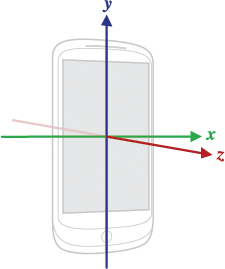
\includegraphics[width=5cm]{gambar/landasan-teori/axis_device.png}
    \caption{Sistem koordinat relatif terhadap perangkat yang digunakan dalam Android SDK (developer.android.com)}
    \label{gambar:koordinat-sensor-android}
\end{figure}

Sensor pada Android dapat diakses dengan membuat \mintinline{java}{SensorManager} yang diinisialisasi dengan \mintinline{java}{getSystemService(Context.SENSOR_SERVICE)}, seperti contoh berikut:

\begin{listing}[h]
    \begin{minted}{java}
        private SensorManager mSensorManager;
        private Sensor sensor;

        mSensorManager = (SensorManager)
        getSystemService(Context.SENSOR_SERVICE)
        sensor = mSensorManager.getDefaultSensor(JENIS_SENSOR)
    \end{minted}
\end{listing}


%------------------------------------------------------------------------------
% Akselerometer
%------------------------------------------------------------------------------
\section{Akselerometer}
Akselerometer adalah sensor yang digunakan untuk mengukur percepatan. Pada akselerometer \textit{Microelectrochemical System (MEMS)}, percepatan diukur dengan mengaitkan massa pada pegas dan melihat penyimpangan massa dari posisi setimbangnya \citep{milette-2012}, seperti yang diilustrasikan pada Gambar~\ref{gambar:akselerometer-mems}.

\begin{figure}[h!]
    \centering
    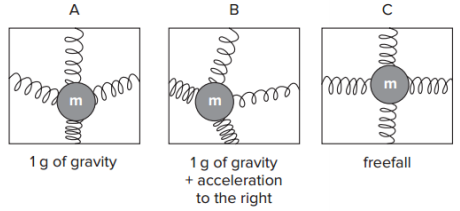
\includegraphics[width=10cm]{gambar/landasan-teori/akselerometer-mems.png}
    \caption{Gaya dikenakan pada massa yang terikat pada pegas \citep{milette-2012}}
    \label{gambar:akselerometer-mems}
\end{figure}

Pada sistem operasi Android, sensor akselerometer dapat diakses dengan menggunakan argumen \mintinline{java}{Sensor.TYPE_ACCELEROMETER} pada metode \mintinline{java}{getDefaultSensor()}, seperti contoh berikut:

\begin{listing}[h]
    \begin{minted}{java}
        private SensorManager mSensorManager;
        private Sensor accelerometer;

        mSensorManager = (SensorManager)
        getSystemService(Context.SENSOR_SERVICE)
        sensor = mSensorManager.getDefaultSensor(Sensor.TYPE_ACCELEROMETER)
    \end{minted}
\end{listing}

Data bacaan sensor disimpan dalam larik multidimensi pada \mintinline{java}{SensorEvent}. Data tersebut dapat dibaca dengan mengimplementasikan metode \textit{callback} \linebreak \mintinline{java}{onSensorChanged(SensorEvent event)}. Nilai bacaan sumbu x, y dan z akselerometer dapat diambil secara berurutan pada larik \mintinline{java}{SensorEvent.values} dengan indeks nol, satu dan dua. Berikut ini contoh pengambilan data sensor akselerometer:

\begin{listing}[h]
    \begin{minted}{java}
        public void onSensorChanged(SensorEvent event) {
            ax = event.values[0]
            ay = event.values[1]
            az = event.values[2]
        }
    \end{minted}
\end{listing}



%------------------------------------------------------------------------------
% Giroskop
%------------------------------------------------------------------------------
\section{Giroskop}
Seperti akselerometer MEMS, giroskop MEMS juga merupakan massa yang dikaitkan pada pegas. Giroskop MEMS digunakan untuk mengukur gaya coriolis yang terjadi karena rotasi. Giroskop MEMS bekerja dengan mendorong massa bolak-balik dalam satu sumbu. Ketika giroskop berputar, gaya coriolis membuat massa menyimpang dari arah getarannya sehingga bergerak ke arah sumbu yang berbeda. Pergerakan ini diukur secara elektrik dengan plat kapasitor, satu plat ditempatkan pada kerangka dan satu plat pada massa yang bergerak. Gaya coriolis hanya berlaku ketika perangkat berputar, sehingga giroskop dapat digunakan untuk mengukur kecepatan sudutnya \citep{milette-2012}.

Pada sistem operasi Android, sensor giroskop dapat diakses dengan menggunakan argumen \mintinline{java}{Sensor.TYPE_GYROSCOPE} pada metode \mintinline{java}{getDefaultSensor()}, seperti contoh berikut:

\begin{listing}[h]
    \begin{minted}{java}
        private SensorManager mSensorManager;
        private Sensor accelerometer;

        mSensorManager = (SensorManager)
        getSystemService(Context.SENSOR_SERVICE)
        sensor = mSensorManager.getDefaultSensor(Sensor.TYPE_GYROSCOPE)
    \end{minted}
\end{listing}

Seperti pada akselerometer, data bacaan sensor disimpan dalam larik multidimensi pada \mintinline{java}{SensorEvent}. Nilai bacaan sumbu x, y dan z giroskop dapat diambil secara berurutan pada larik \mintinline{java}{SensorEvent.values} dengan indeks nol, satu dan dua.


%------------------------------------------------------------------------------
% Pembelajaran Mesin
%------------------------------------------------------------------------------
\section{Pembelajaran Mesin}
Pembelajaran mesin adalah kemampuan komputer untuk beradaptasi dengan keadaan baru dan mendeteksi serta meramalkan kemungkinan pola. Terdapat tiga jenis \textit{feedback} yang menentukan tiga jenis utama pembelajaran mesin. \textit{Unsupervised learning} mempelajadi pola pada input meskiput tidak disediakan \textit{feedback} secara eksplisit, \textit{supervised learning} mengamati contoh pasangan input-output dan mempelajari fungsi yang memetakan dari input ke output, sedangkan \textit{reinforcement learning} melakukan pembelajaran dari rangkaian penghargaan atau hukuman \citep{Russell:2009:AIM:1671238}. Salah satu masalah yang berusaha diselesaikan proses pembelajaran mesin adalah klasifikasi, yaitu ketika output adalah satu dari himpunan terhingga nilai-nilai.


%------------------------------------------------------------------------------
% Deep Learning
%------------------------------------------------------------------------------
\section{Deep Learning}
Dalam pembelajaran mesin, performa suatu algoritma sangat bergantung pada representasi dari data yang digunakan. Setiap informasi yang menjadi representasi data disebut sebagai fitur.

Salah satu masalah dalam pembelajaran mesin adalah sulitnya mengetahui fitur-fitur apa saja yang harus diekstrak dari suatu set data. Masalah ini dapat diatasi dengan menggunakan pembelajaran mesin bukan hanya untuk menemukan pemetaan dari representasi ke output, tapi juga menemukan representasi itu sendiri. Pendekatan ini dikenal dengan \textit{representation learning} \citep{goodfellow-2016}.

Pada aplikasinya di dunia nyata, \textit{representation learning} sering mengalami kesulitan dalam menemukan representasi dari data yang kompleks. \textit{Deep learning} mengatasi masalah ini dengan membuat representasi yang disusun oleh representasi-representasi lain yang lebih sederhana.

\citeauthor{goodfellow-2016} mendefinisikan \textit{deep learning} sebagai salah satu jenis pembelajaran mesin yang memiliki kemampuan dan fleksibilitas tinggi dengan belajar merepresentasikan dunia sebagai hierarki konsep yang bersarang. Setiap konsep didefinisikan oleh kaitannya terhadap konsep-konsep yang lebih sederhana dan representasi yang lebih abstrak dihitung berdasarkan representasi yang kurang abstrak. Perbandingan \textit{deep learning} dengan sistem inteligensia buatan lainnya dapat dilihat pada Gambar~\ref{gambar:perbandingan-ai}.

\begin{figure}
    \centering
    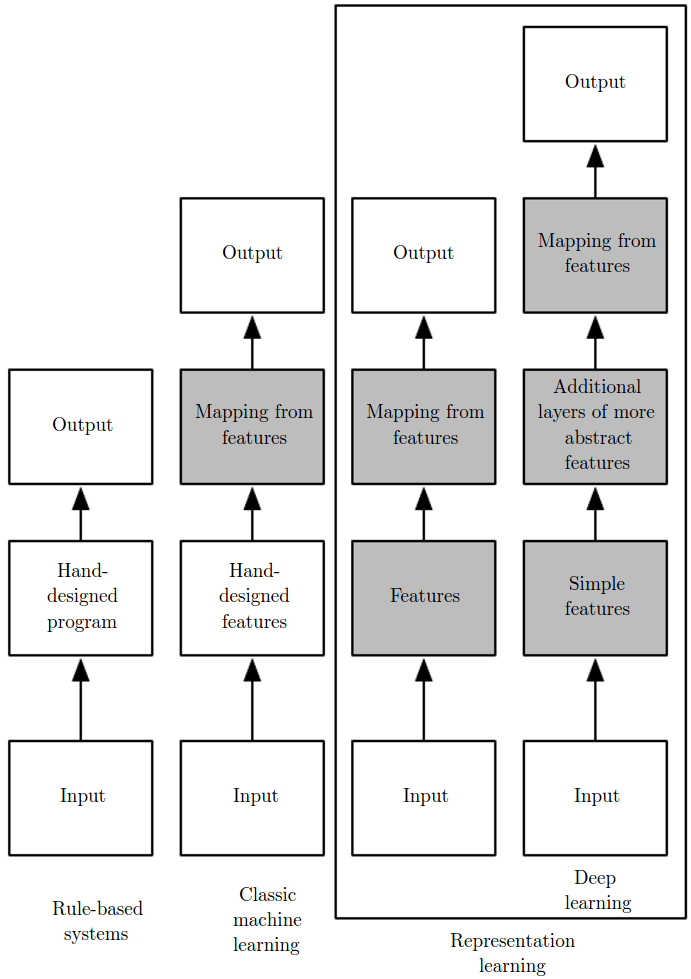
\includegraphics[width=12cm]{gambar/landasan-teori/perbandingan-ai.png}
    \caption{Perbandingan sistem AI. Kotak berwarna abu-abu menunjukkan komponen yang dapat belajar dari data \citep{goodfellow-2016}}
    \label{gambar:perbandingan-ai}
\end{figure}


%------------------------------------------------------------------------------
% Convolutional Neural Network
%
% TODO:
% - Apa perlu membahas sparse interactions, paramater sharing dan
%   equivariant representations?
% - Terjemahan paragraf pertama
%
%------------------------------------------------------------------------------
\section{Convolutional Neural Network}
Convolutional neural network (CNN) adalah jenis jaringan saraf untuk mengolah data \textit{grid-like topology}, seperti \textit{time-series data}, yang dapat dianggap sebagai grid 1D dengan sample pada interval tertentu, dan data citra, yang dapat dianggap sebagai 2D grid of pixels. CNN menggunakan operasi konvolusi untuk menggantikan operasi perkalian matriks pada setidaknya satu lapisan \citep{goodfellow-2016}. Operasi konvolusi dinotasikan sebagai:

\begin{equation}
    \label{eq:konvolusi}
    s(i) = (x * w)(i)
\end{equation}

Dalam terminologi CNN $x$ merupakan input, $w$ adalah kernel, dan outputnya disebut sebagai \textit{feature map}. Input $x$ merupakan larik multidimensi (tensor) parameter yang disesuaikan oleh algoritma pembelajaran.

Saat bekerja dengan data diskrit, persamaan~\ref{eq:konvolusi} dapat ditulis sebagai persamaan konvolusi diskrit:

\begin{equation}
    \label{eq:konvolusi-diskrit}
    s(i) = (x * w)(i) = \sum_{a=-\infty}^{\infty} x(a) w(i - a)
\end{equation}

Pada umumnya, konvolusi digunakan pada lebih dari satu sumbu. Misalnya, jika input adalah data dua dimensi seperti pada Gambar~\ref{gambar:konvolusi-2d}, maka digunakan kernel dua dimensi:
\begin{equation}
    \label{eq:konvolusi-2d}
    S(i,j) = (I * K)(i,j) = \sum_{m}\sum_{n}I(m,n)K(i-m, j-n)
\end{equation}

\begin{figure}[t!]
    \centering
    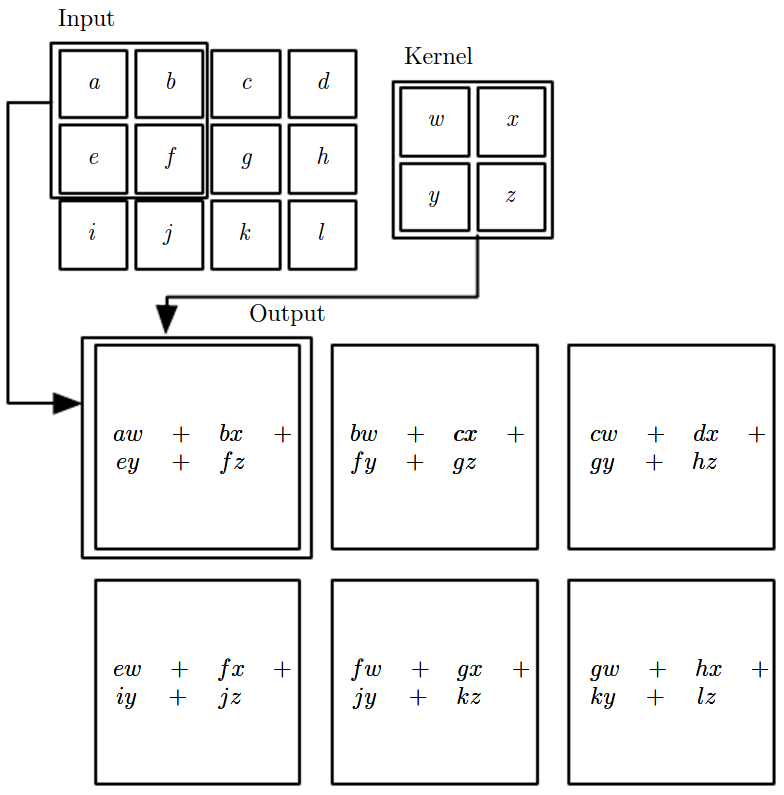
\includegraphics[width=10cm]{gambar/landasan-teori/konvolusi-2d.png}
    \caption{Contoh operasi konvolusi pada data dua dimensi \citep{goodfellow-2016}}
    \label{gambar:konvolusi-2d}
\end{figure}


%------------------------------------------------------------------------------
% Recurrent Neural Network
%
% TODO:
% - Ganti gambar RNN
%------------------------------------------------------------------------------
\section{Recurrent Neural Network}
Recurrent Neural Network (RNN) adalah keluarga jaringan saraf untuk memproses data sekuensial. RNN merupakan \textit{feedforward neural network} dengan hubungan yang berputar. Gambar~\ref{gambar:rnn} menunjukkan graf RNN dan graf yang setara namun telah dibentangkan berdasarkan langkah waktu. RNN dapat memetakan riwayat dari input sebelumnya ke setiap output. Dengan kata lain, koneksi yang berulang ini memungkinkan memori dari input sebelumnya tersimpan dalam kondisi internal jaringan, sehingga mempengaruhi output~\citep{graves-2012}.

\begin{figure}
    \centering
    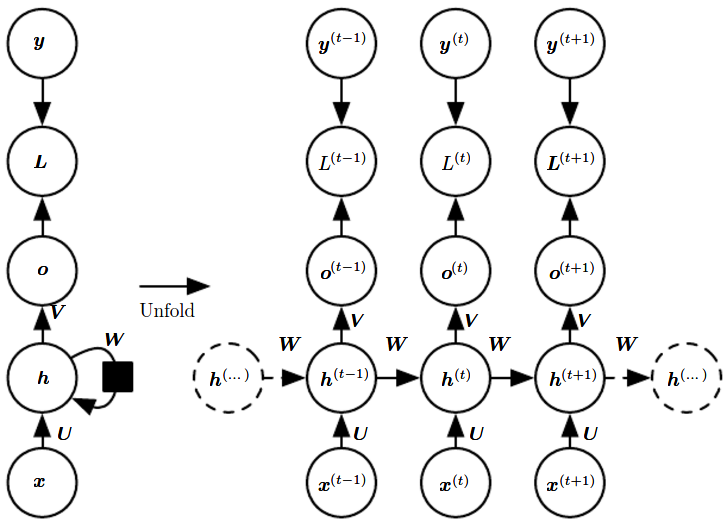
\includegraphics[width=10cm]{gambar/landasan-teori/rnn.png}
    \caption{Graf komputasi \textit{recurrent neural network} \citep{goodfellow-2016}}
    \label{gambar:rnn}
\end{figure}

Jika pada RNN dengan output diskrit diberikan output $\pmb{o}$ sebagai \textit{unormalized log probabilities} untuk setiap nilai yang mungkin dari variabel diskrit, operasi softmax dapat dilakukan sebagai langkah \textit{post-processing} untuk memperoleh vektor probabilitas normal $\pmb{\hat{y}}$ pada output. Propagasi maju dimulai dengan memberikan kondisi awal $\pmb{h}^{(0)}$. Lalu, pada setiap langkah waktu dari $t = 1$ sampai $t = \tau$, dilakukan perhitungan berikut:

\begin{align}
    \pmb{a}^{(t)} &= \pmb{b} + \pmb{Wh}^{(t-1)} + \pmb{Ux}^{(t)} \\
    \pmb{h}^{(t)} &= \tanh(\pmb{a}^{(t)}) \\
    \pmb{o}^{(t)} &= \pmb{c} + \pmb{Vh}^{(t)} \\
    \pmb{\hat{y}}^{(t)} &= softmax(\pmb{o}^{(t)})
\end{align}

\noindent
dengan $\pmb{b}$, $\pmb{c}$ vektor bias dan $\pmb{U}$, $\pmb{V}$, $\pmb{W}$ matriks bobot untuk hubungan input ke hidden, hidden ke output dan hidden ke hidden. Total \textit{loss} untuk pasangan $\pmb{x}$ dan $\pmb{y}$ dihitung dengan menjumlahkan \textit{loss} dari seluruh langkah waktu \citep{goodfellow-2016}.



%------------------------------------------------------------------------------
% Long Short-Term Memory
%------------------------------------------------------------------------------
\section{Long Short-Term Memory}
Long Short-Term Memory (LSTM) adalah salah satu jenis RNN bergerbang. Arsitektur LSTM terdiri dari kumpulan jaringan dengan hubungan internal berulang yang disebut dengan blok memori. Setiap blok memiliki satu atau lebih sel memori \textit{self-loop} dan tiga unit pengali, yaitu gerbang \textit{input, output} dan \textit{forget} \citep{graves-2012}.

\begin{figure}
    \centering
    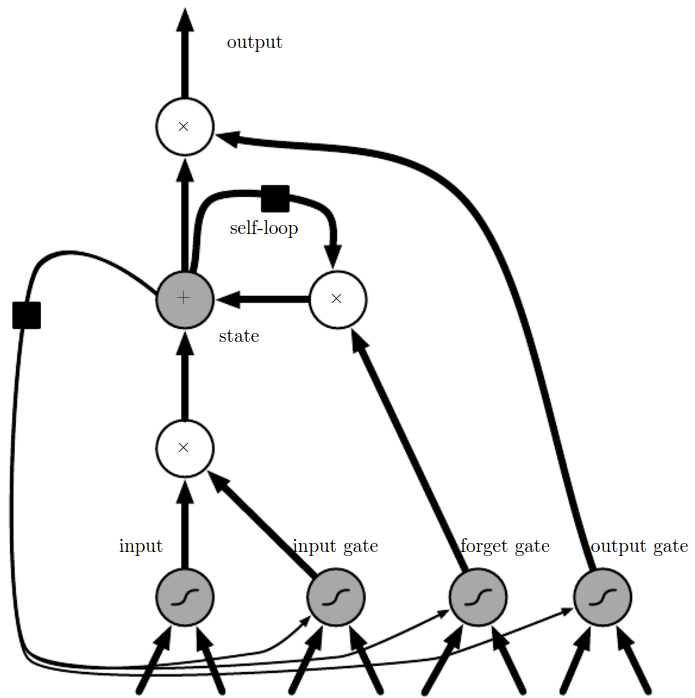
\includegraphics[width=10cm]{gambar/landasan-teori/lstm.png}
    \caption{Graf komputasi sel LSTM \citep{goodfellow-2016}}
    \label{gambar:lstm}
\end{figure}

Pada LSTM, bobot \textit{self-loop} dikendalikan oleh unit gerbang \textit{forget} $f_{i}^{(t)}$ (untuk langkah waktu $t$ dan sel $i$) yang memberikan nilai bobot antara 0 dan 1 melalui unit sigmoid:

\begin{equation}
    f_{i}^{(t)} = \sigma\left(b_{i}^{f} + \sum_{j} U_{i,j}^{f} x_{j}^{(t)} + \sum_{j} W_{i,j}^{f} h_{j}^{(t-1)}\right)
\end{equation}

\noindent
dengan $\pmb{x}^{(t)}$ vektor input saat ini, $\pmb{h}^{(t)}$ vektor \textit{hidden layer} saat ini yang berisi output dari seluruh sel LSTM, dan $\pmb{b}^{f}$, $\pmb{U}^{f}$, $\pmb{W}^{f}$ adalah bias, bobot input dan bobot pengulangan untuk gerbang \textit{forget}. Kondisi internal sel LSTM $s_{i}^{(t)}$ diperbarui sebagai berikut:

\begin{equation}
    s_{i}^{(t)} = f_{i}^{(t)}  s_{i}^{(t-1)} + g_{i}^{(t)} \sigma\left(b_{i} + \sum_{j} U_{i,j} x_{j}^{(t)} + \sum_{j} W_{i,j} h_{j}^{(t-1)} \right)
\end{equation}

\noindent
dengan $\pmb{b}, \pmb{U}$ dan $\pmb{W}$ sebagai bias, bobot input dan bobot pengulangan ke sel LSTM\@. Unit gerbang input eksternal $g_{i}^{(t)}$ dihitung dengan:

\begin{equation}
    g_{i}^{(t)} = \sigma\left(b_{i}^{g} + \sum_{j} U_{i,j}^{g} x_{j}^{(t)} + \sum_{j} W_{i,j}^{g} h_{j}^{(t-1)}\right)
\end{equation}

Output LSTM $h_{i}^{(t)}$ dapat dimatikan melalui gerbang output $q_{i}^{(t)}$, yang juga menggunakan unit sigmoid:

\begin{align}
    \label{eq:output-lstm}
    h_{i}^{(t)} &= \tanh\left(s_{i}^{(t)}\right) q_{i}{(t)} \\
    q_{i}^{(t)} &= \sigma\left(b_{i}^{o} + \sum_{j} U_{i,j}^{o} x_{j}^{(t)} + \sum_{j} W_{i,j}^{o} h_{j}^{(t-1)} \right)
\end{align}

\noindent
dengan $\pmb{b}^{o}, \pmb{U}^{o}$ dan $\pmb{W}^{o}$ sebagai bias, bobot input dan bobot pengulangan \citep{goodfellow-2016}.

% \section{Stochastic Gradient Descent}


%------------------------------------------------------------------------------
% Backpropagation Through Time
%------------------------------------------------------------------------------
\section{Backpropagation Through Time}
Kebanyakan algoritma \textit{deep learning} membutuhkan proses optimasi, yaitu proses meminimalkan atau memaksimalkan suatu fungsi $f(\pmb{x})$ dengan mengubah $\pmb{x}$. Fungsi yang akan diminimalkan atau dimaksimalkan disebut fungsi objektif. Dalam kasus meminimalkan, fungsi objektif bisa juga disebut \textit{cost function}, \textit{loss function} atau \textit{error function} \citep{goodfellow-2016}.

\citeauthor{goodfellow-2016} menambahkan, jika diberikan fungsi $y = f(x)$ dengan $x$ dan $y$ bilangan real, derivatif dari fungsi ini adalah gradien $f(x)$ pada titik $x$, dinotasikan dengan $f'(x)$ atau $\frac{dy}{dx}$. Fungsi $f(x)$ dapat diminimalkan dengan membuat perubahan $x$ ke arah yang berlawanan dengan derivatifnya. Cara ini disebut \textit{gradient descent}, diilustrasikan pada Gambar~\ref{gambar:gradient-descent}.

\begin{figure}
    \centering
    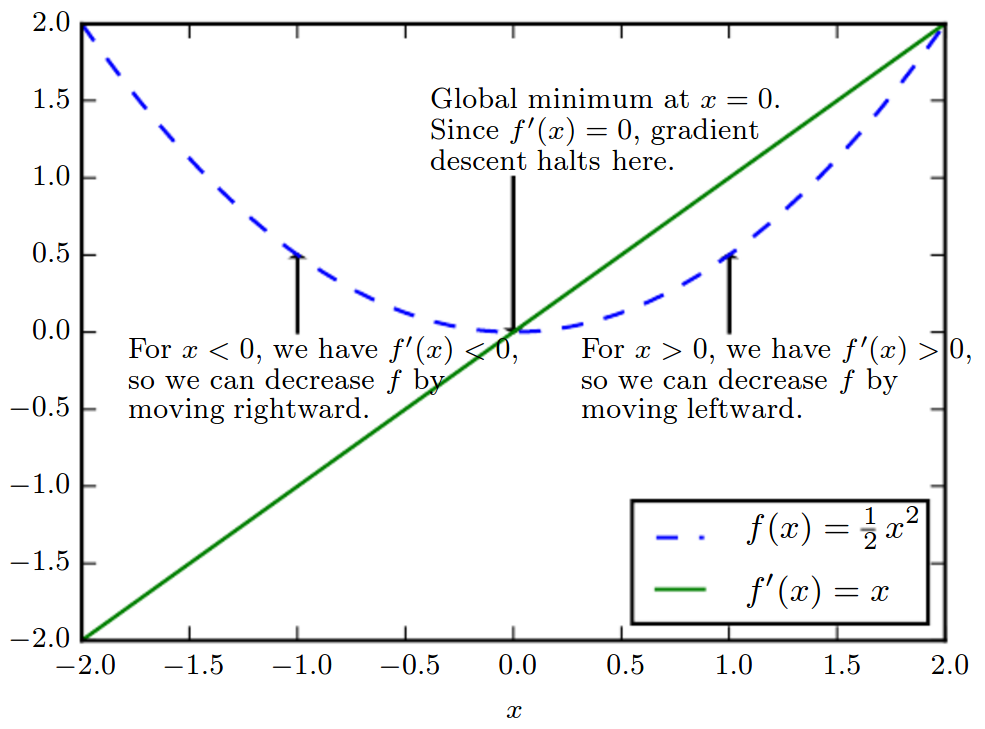
\includegraphics[width=12cm]{gambar/landasan-teori/gradient-descent.png}
    \caption{\textit{Gradient descent} menggunakan derivatif untuk meminimalkan sebuah fungsi \citep{goodfellow-2016}}.
    \label{gambar:gradient-descent}
\end{figure}

Ketika \textit{feedforward neural network} menerima input $\pmb{x}$ dan menghasilkan output $\pmb{\hat{y}}$, informasi mengalir maju melalui jaringan. Input $\pmb{x}$ menyediakan informasi awal yang merambat ke \textit{hidden unit} pada setiap layer hingga akhirnya menghasilkan $\pmb{\hat{y}}$. Proses ini disebut \textit{forward propagation}. Dalam proses latihan, \textit{forward propagation} dapat terus maju sampai menghasilkan nilai skalar \textit{cost} $J(\theta)$. Algoritma \textit{backpropagation} memungkinkan informasi dari \textit{cost} mengalir mundur melalui jaringan untuk menghitung gradiennya \citep{goodfellow-2016}.

\textit{Backpropagation} menghitung derivatif fungsi dengan aturan rantai kalkulus. \citet{nielsen-2015} mendefinisikan algoritma backpropagation dalam lima langkah:
\begin{enumerate}
    \item Input x: Atur aktivasi $a^{l}$ untuk lapisan input
    \item Feedforward: Untuk setiap $l = 2, 3, \ldots, L$ hitung $z^{l} = w^{l} a^{l-1} + b^{l}$ dan $a^{l} = \sigma (z^{l})$
    \item Output error $\delta^{L}$: Hitung vektor $\delta^{L} = \nabla_{a} C \odot \sigma ' (z^{L})$
    \item Rambatkan error ke belakang: Untuk setiap $l = L-1, L-2, \ldots, 2$ hitung $\delta^{l} = ({(w^{l+1})}^{T} \delta^{l+1}) \odot \sigma' (z^{l})$
    \item Output: Hitung gradient dari \textit{cost function} dengan $\frac{\partial C}{\partial w_{jk}^{l}} = a_{k}^{l-1} \delta_{j}^{l}$ dan $\frac{\partial C}{\partial b_{j}^{l}} = \delta_{j}^{l}$
\end{enumerate}

\noindent
dengan $L$ jumlah lapisan dalam jaringan, $C$ \textit{cost function}, $w_{jk}^{l}$ bobot koneksi dari neuron ke-$k$ pada lapisan $(l-1)$ ke neuron ke-$j$ pada lapisan $l$ dan $b_{j}^{l}$ bias neuron ke-$j$ pada lapisan $l$.

Pada RNN, aktivasi \textit{hidden layer} tidak hanya mempengaruhi \textit{loss function} pada \textit{output layer}, namun juga mempengaruhi \textit{hidden layer} pada langkah waktu selanjutnya. Maka, gradien dihitung dengan menggunakan \textit{backpropagation} pada graf yang telah dibentangkan. Metode ini bernama \textit{backpropagation through time (BPTT)} \citep{graves-2012}.


%------------------------------------------------------------------------------
% Tensorflow
%------------------------------------------------------------------------------
\section{TensorFlow}
TensorFlow adalah pustaka sumber terbuka pembalajaran mesin. TensorFlow melakukan komputasi yang dideskripsikan dengan model aliran data dan memetakannya ke berbagai jenis perangkat keras berbeda, mulai dari melakukan pengambilan kesimpulan pada perangkat bergerak seperti Android dan iOS, pelatihan dan sistem pengambilan keputusan berukuran sedang menggunakan satu mesin yang terdiri dari satu atau lebih kartu GPU sampai ke sistem pelatihan berskala besar yang berjalan pada ratusan mesin khusus dengan ribuan GPU \citep{abadi-2015}.

\begin{figure}
    \centering
    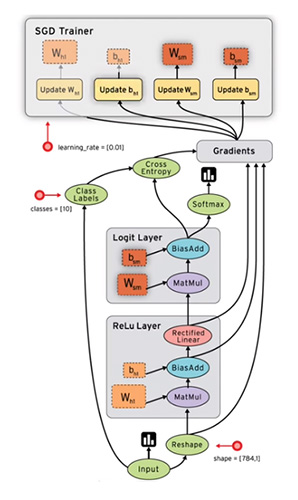
\includegraphics[width=6cm]{gambar/landasan-teori/tensorflow.jpg}
    \caption{Contoh graf aliran data dalam TensorFlow (tensorflow.com)}
    \label{gambar:tensorflow}
\end{figure}

Graf aliran data dalam TensorFlow mendeskripsikan komputasi matematis dengan graf \textit{node} dan \textit{edge} terarah. \textit{Edge} memuat array multidimensi berukuran dinamis yang disebut dengan tensor. Para \textit{node} bekerja secara asinkron dan paralel ketika seluruh tensor pada \textit{edge} yang masuk telah tersedia. Contoh graf aliran data pada TensorFlow dapat dilihat pada Gambar~\ref{gambar:tensorflow}. Aliran data tersebut direpresentasikan oleh TensorFlow melalui API yang tersedia untuk bahasa Python, C++, Java dan Go.



\chapter{METODE PENELITIAN}


\input{bab/5-hasil-penelitian.tex}
\input{bab/6-kesimpulan.tex}


\bibliography{pustaka}

\end{document}
